\section{Theorie}
\label{sec:Theorie}

Um einen Brechungsindex zu berechnen benötigt es Linsen, die aus einem anderen Material bestehen als Luft, sodass ein Übergang der Brechungsindizes entsteht.
\subsection{Brechung}
Das Brechungsgesetz beschreibt den Vorgang, wenn ein Lichtstrahl aus einem Medium in ein Medium einer anderen Beschaffenheit übergeht.
Dabei sorgen die Brechungsindizes der Medien für den Grad der Brechung.\\
Trifft ein Lichtstrahl auf eine Linse, so wird dieser beim Eintritt und Austritt gebrochen.
Abhängig davon, ob es eine Sammellinse ist oder eine Zerstreuungslinse, wird der Strahl anders abgelenkt.\\
Die \autoref{eq:break} zeigt das Brechungsgesetz, wobei $n_{1,2}$ die Brechungsindizes und $\phi_{1,2}$ die auftretenden Winkel sind.

\begin{equation}
    n_1 \sin{\phi_1} = n_2 \sin{\phi_2}
    \label{eq:break}
\end{equation}

\subsection{Linsen}
Bei Sammellinsen ist die Brennweite $f$, sowie die Bildweite $b$ positiv, sodass ein reelles Bild des Objektes entsteht.
In \autoref{fig:sammel} sind die Strahlengänge, sowie die Abstände der Gegenstandsweite $g$ und der Bildweite $b$ dargestellt.

\begin{figure}[htbp]
    \centering
    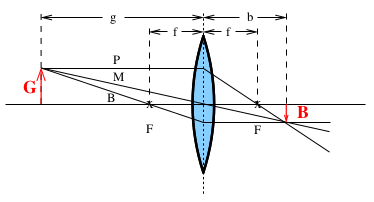
\includegraphics[scale=0.5]{Data/Sammeldia.png}
    \caption{Darstellung des Strahlenverlaufs einer dünnen Sammellinse.}
    \label{fig:sammel}
\end{figure}

Wird eine Zerstreuungslinse betrachtet, ändern sich die Vorzeichen der Brenn- und Bildweite, sodass ein virtuelles Bild entsteht.
Zusammen mit den Strahlengängen ist dies in \autoref{fig:streu} dargestellt.

\begin{figure}[htbp]
    \centering
    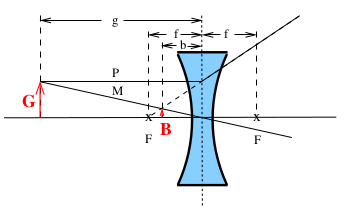
\includegraphics[scale=0.5]{Data/Streudia.png}
    \caption{Darstellung des Strahlungsverlaufs einer Zerstreuungslinse.}
    \label{fig:streu}
\end{figure}

\subsection{Abbildungsgesetz}
Mittels der Bildkonstruktion der verschiedenen Linsen und den Strahlungssätzen, lässt sich auf das Abbildungsgesetz schließen:

\begin{equation}
    V=\frac{B}{G}=\frac{b}{g}
    \label{eq:abb}
\end{equation}

Mithilfe \autoref{eq:abb} lässt sich für dünne Sammellinsen ein Zusammenhang aus Brennweite $f$ und der Bild- und Gegenstandsweite bestimmen:

\begin{equation}
    \frac{1}{f} = \frac{1}{b}\ +\ \frac{1}{g}
    \label{eq:linse}
\end{equation}

Dieser Zusammenhang ist die Linsengleichung.\\
Der Ausdruck $\frac{1}{f}$ wird definiert als die Brechkraft $D$.
Bei mehreren Sammellinsen hintereinander kann dann die gesamte Brechkraft als Summe aller einzelnen Brechkräfte errechnet werden:

\begin{equation}
    D_{ges} = \sum_i^N D_i
\end{equation}

\subsection{Bessel und Abbe}
Die Bestimmung der Brennweite über die Methode von Bessel basiert auf zwei Linsenpositionen und dessen Bild- und Gegenstandsweite.
In beiden Positionen ergibt sich ein klares Bild.\\
Zur Berechnung gilt $e = g_1\ +\ b_1=g_2\ +\ b_2$ und $d = g_1\ -\ b_1=g_2\ -\ b_2$.

\begin{equation}
    f = \frac{e^2\ +\ d^2}{4e}
    \label{eq:bessel}
\end{equation}

Die Methode von Abbe beinhaltet ein Linsensystem, dessen genaue Streuebenen nicht erkennbar sind.
Über einen Referenzpunkt A können jedoch die Bildweite $b'$ und die Gegenstandsweite $g'$ gemessen werden.
$b'$ und $g'$ sind Funktionen der Brennweite und über die Terme:

\begin{equation}
    b' = f\cdot(1+V)+h'
    \label{eq:abbe}
\end{equation}
\begin{equation*}
    g' = f\cdot(1+\frac{1}{V})+h
\end{equation*}

definiert.